% Schematic overview of the companion paper: four aspects of active control.
% Compile standalone:  pdflatex fig_overview.tex
% Included in draft.tex as fig_overview.pdf.
\documentclass[tikz,border=4pt]{standalone}
\usepackage{amssymb}
\usepackage[scaled=0.92]{helvet}
\renewcommand{\familydefault}{\sfdefault}
\usetikzlibrary{arrows.meta,fit,backgrounds,calc}

\definecolor{passive}{HTML}{6B6B6B}
\definecolor{active}{HTML}{D55E00}
\definecolor{panel}{HTML}{F4F4F4}
\definecolor{neck}{HTML}{3B6EA5}

\tikzset{
  ptitle/.style={font=\bfseries, anchor=north west},
  note/.style={font=\scriptsize, align=left, anchor=north west},
  res/.style={font=\scriptsize\itshape, align=left, anchor=north west, text=black!80},
  flow/.style={-{Stealth[length=2.4mm]}, line width=0.9pt, black!60},
  lever/.style={draw=active, rounded corners=3pt, fill=white, font=\scriptsize, align=center,
                text width=2.55cm, inner sep=3pt},
  neckbox/.style={draw=neck, rounded corners=3pt, fill=neck!8, font=\scriptsize, align=center,
                  text width=2.85cm, inner sep=3pt},
  ep/.style={minimum width=0.42cm, minimum height=0.42cm, inner sep=0pt, draw=white},
}
\hyphenpenalty=10000 \exhyphenpenalty=10000
\newcommand{\Cv}{\textit{C}}

\begin{document}
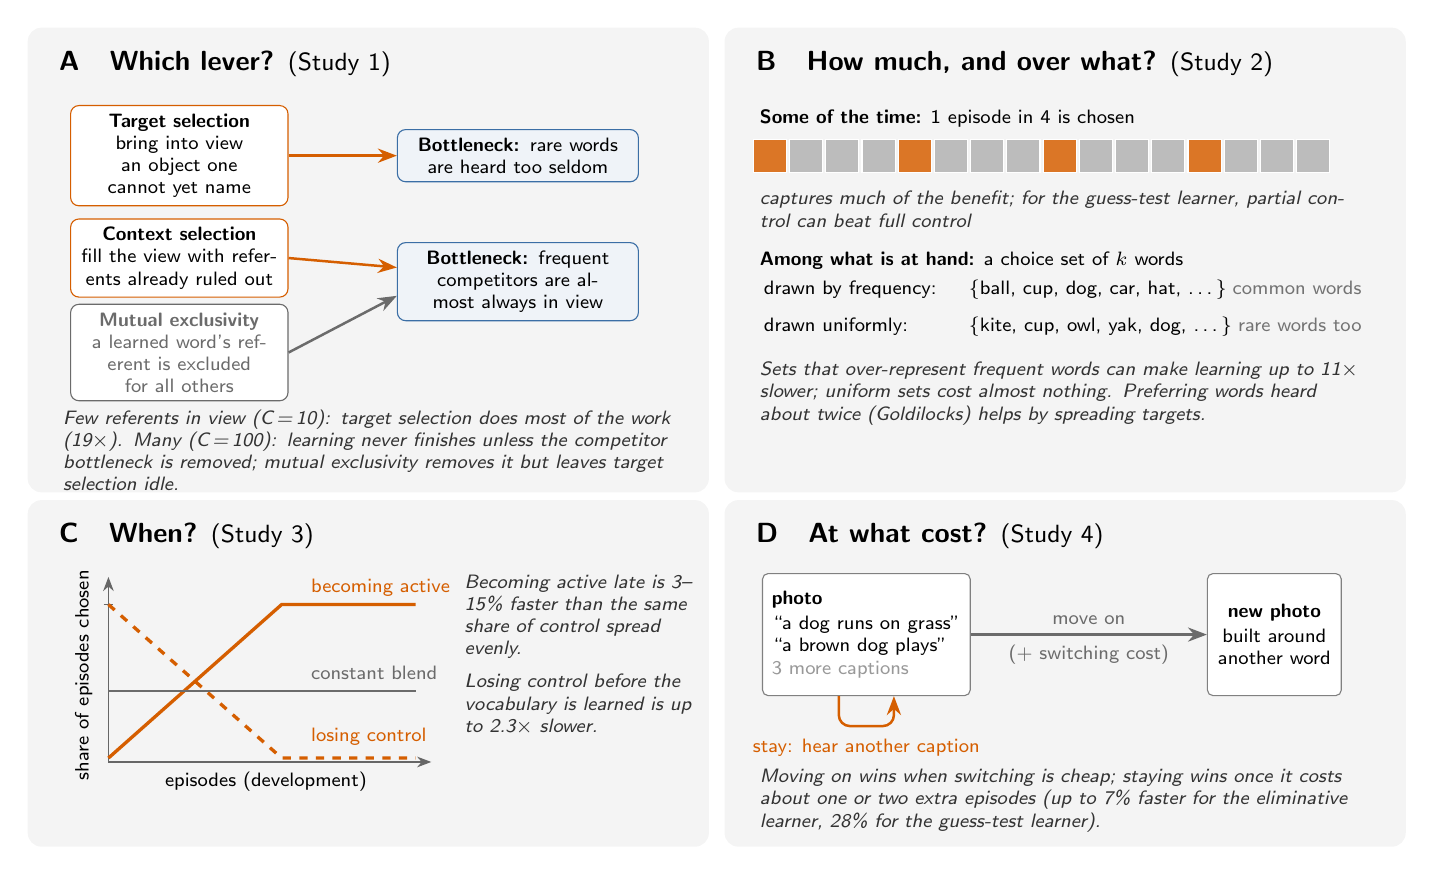
\begin{tikzpicture}

% =====================================================================
% Panel A: which lever? (Study 1)
% =====================================================================
\node[ptitle] (At) at (0, 11.0) {A\quad Which lever? \normalfont\small(Study 1)};

\node[neckbox] (n1) at (5.95, 9.55) {\textbf{Bottleneck:} rare words are heard too seldom};
\node[neckbox] (n2) at (5.95, 7.95) {\textbf{Bottleneck:} frequent competitors are almost always in view};

\node[lever] (l1) at (1.65, 9.55) {\textbf{Target selection}\\bring into view an object one cannot yet name};
\node[lever] (l2) at (1.65, 8.25) {\textbf{Context selection}\\fill the view with referents already ruled out};
\node[lever, draw=passive, text=passive] (l3) at (1.65, 7.05) {\textbf{Mutual exclusivity}\\a learned word's referent is excluded for all others};

\draw[flow, active] (l1.east) -- (n1.west);
\draw[flow, active] (l2.east) -- ($(n2.west)+(0,0.18)$);
\draw[flow, passive] (l3.east) -- ($(n2.west)+(0,-0.18)$);

\node[res, text width=7.9cm] at (0.05, 6.45)
  {Few referents in view (\Cv\,=\,10): target selection does most of the work (19$\times$). Many (\Cv\,=\,100): learning never finishes unless the competitor bottleneck is removed; mutual exclusivity removes it but leaves target selection idle.};

\begin{scope}[on background layer]
  \node[fill=panel, rounded corners=5pt, fit={(At) (-0.1,5.45) (8.2,11.0)}, inner sep=5pt] {};
\end{scope}

% =====================================================================
% Panel B: how much control, and over what? (Study 2)
% =====================================================================
\node[ptitle] (Bt) at (8.85, 11.0) {B\quad How much, and over what? \normalfont\small(Study 2)};

% partial autonomy: a strip of episodes, a quarter of them active
\node[note] at (8.9, 10.25) {\textbf{Some of the time:} 1 episode in 4 is chosen};
\foreach \i in {0,...,15} {
  \pgfmathsetmacro{\isact}{mod(\i,4)==0 ? 1 : 0}
  \ifdim\isact pt=1pt
    \node[ep, fill=active!85] at (9.15 + 0.46*\i, 9.55) {};
  \else
    \node[ep, fill=passive!45] at (9.15 + 0.46*\i, 9.55) {};
  \fi
}
\node[res, text width=7.7cm] at (8.9, 9.22)
  {captures much of the benefit; for the guess-test learner, partial control can beat full control};

% bounded choice: what's at hand
\node[note] at (8.9, 8.45) {\textbf{Among what is at hand:} a choice set of $k$ words};
\node[font=\scriptsize, anchor=west] at (8.95, 7.85) {drawn by frequency:};
\node[font=\scriptsize, anchor=west] at (11.55, 7.85) {\{ball, cup, dog, car, hat, \dots\}\;\textcolor{black!55}{common words}};
\node[font=\scriptsize, anchor=west] at (8.95, 7.38) {drawn uniformly:};
\node[font=\scriptsize, anchor=west] at (11.55, 7.38) {\{kite, cup, owl, yak, dog, \dots\}\;\textcolor{black!55}{rare words too}};
\node[res, text width=7.7cm] at (8.9, 7.05)
  {Sets that over-represent frequent words can make learning up to 11$\times$ slower; uniform sets cost almost nothing. Preferring words heard about twice (Goldilocks) helps by spreading targets.};

\begin{scope}[on background layer]
  \node[fill=panel, rounded corners=5pt, fit={(Bt) (8.75,5.45) (17.05,11.0)}, inner sep=5pt] {};
\end{scope}

% =====================================================================
% Panel C: when? (Study 3)
% =====================================================================
\node[ptitle] (Ct) at (0, 5.0) {C\quad When? \normalfont\small(Study 3)};

\begin{scope}[shift={(0.75, 1.85)}]
  \draw[-{Stealth[length=1.8mm]}, black!60] (0,0) -- (4.1,0);
  \draw[-{Stealth[length=1.8mm]}, black!60] (0,0) -- (0,2.35);
  \node[font=\scriptsize, anchor=north] at (2.0,0) {episodes (development)};
  \node[font=\scriptsize, rotate=90, anchor=south] at (-0.08,1.1) {share of episodes chosen};
  \draw[black!60] (-0.06,2.0) -- (0.06,2.0);
  % forward ramp
  \draw[active, line width=1.2pt] (0,0.05) -- (2.2,2.0) -- (3.9,2.0);
  % reverse ramp
  \draw[active, line width=1.2pt, dashed] (0,2.0) -- (2.2,0.05) -- (3.9,0.05);
  % constant blend with the same share
  \draw[passive, line width=1.0pt] (0,0.9) -- (3.9,0.9);
  \node[font=\scriptsize, text=active, anchor=west] at (2.45,2.22) {becoming active};
  \node[font=\scriptsize, text=active, anchor=west] at (2.45,0.32) {losing control};
  \node[font=\scriptsize, text=passive, anchor=west] at (2.45,1.13) {constant blend};
\end{scope}

\node[res, text width=2.95cm] at (5.15, 4.35)
  {Becoming active late is 3--15\% faster than the same share of control spread evenly.\\[4pt]
   Losing control before the vocabulary is learned is up to 2.3$\times$ slower.};

\begin{scope}[on background layer]
  \node[fill=panel, rounded corners=5pt, fit={(Ct) (-0.1,0.95) (8.2,5.0)}, inner sep=5pt] {};
\end{scope}

% =====================================================================
% Panel D: at what cost? (Study 4)
% =====================================================================
\node[ptitle] (Dt) at (8.85, 5.0) {D\quad At what cost? \normalfont\small(Study 4)};

% current photo with captions
\node[draw=black!50, fill=white, rounded corners=2pt, minimum width=2.3cm, minimum height=1.55cm,
      font=\scriptsize, align=left, anchor=north west] (photo) at (9.05, 4.25)
  {\textbf{photo}\\[1pt] ``a dog runs on grass''\\``a brown dog plays''\\\textcolor{black!40}{3 more captions}};
% new photo
\node[draw=black!50, fill=white, rounded corners=2pt, minimum width=1.7cm, minimum height=1.55cm,
      font=\scriptsize, align=center, anchor=north west] (newp) at (14.7, 4.25)
  {\textbf{new photo}\\[1pt]built around\\another word};

\draw[flow, active, rounded corners=4pt] ($(photo.south)+(-0.35,0)$) -- ++(0,-0.38) -- ++(0.7,0) -- ($(photo.south)+(0.35,0)$);
\node[font=\scriptsize, text=active, anchor=north] at ($(photo.south)+(0,-0.42)$) {stay: hear another caption};
\draw[flow, passive] (photo.east) -- node[above, font=\scriptsize, text=passive] {move on} node[below, font=\scriptsize, text=passive] {(+ switching cost)} (newp.west);

\node[res, text width=7.7cm] at (8.9, 1.88)
  {Moving on wins when switching is cheap; staying wins once it costs about one or two extra episodes (up to 7\% faster for the eliminative learner, 28\% for the guess-test learner).};

\begin{scope}[on background layer]
  \node[fill=panel, rounded corners=5pt, fit={(Dt) (8.75,0.95) (17.05,5.0)}, inner sep=5pt] {};
\end{scope}

\end{tikzpicture}
\end{document}
